% !TEX encoding = UTF-8 Unicode

\documentclass[a4paper]{article}

\usepackage{color}
\usepackage{url}
\usepackage[T2A]{fontenc} % enable Cyrillic fonts
\usepackage[utf8]{inputenc} % make weird characters work
\usepackage{graphicx}

\usepackage[english,serbian]{babel}
%\usepackage[english,serbianc]{babel} %ukljuciti babel sa ovim opcijama, umesto gornjim, ukoliko se koristi cirilica

\usepackage[unicode]{hyperref}
\hypersetup{colorlinks,citecolor=green,filecolor=green,linkcolor=blue,urlcolor=blue}

%\newtheorem{primer}{Пример}[section] %ćirilični primer
\newtheorem{primer}{Primer}[section]

\begin{document}

\title{Naslov seminarskog rada\\ \small{Seminarski rad u okviru kursa\\Tehničko i naučno pisanje\\ Matematički fakultet}}

\author{Ime i prezime autora\\ kontakt email adresa autora}
\date{24.~oktobar 2017.}
\maketitle

\abstract{
U ovom tekstu je ukratko prikazana osnovna forma seminarskog rada. Obratite pažnju da je pored ove .pdf datoteke, u prilogu i odgovarajuća .tex datoteka, kao i .bib datoteka korišćena za generisanje literature. Na prvoj strani seminarskog rada su naslov, apstrakt i sadržaj, i to sve mora da stane na prvu stranu! Kako bi Vaš seminarski zadovoljio standarde i očekivanja, koristite uputstva i materijale sa predavanja na temu pisanja seminarskih radova. Ovo je samo šablon koji se odnosi na fizički izgled seminarskog rada (šablon koji \emph{morate} da ispoštujete!) kao i par tehničkih pomoćnih uputstava. 

\tableofcontents

\newpage

\section{Uvod}
\label{sec:uvod}
Kada budete predavali seminarski rad, imenujete datoteke tako da sadrže temu seminarskog rada, kao i prezimena članova grupe. Predaja seminarskih radova biće isključivo preko veb forme, a NE slanjem mejla. Link na formu će biti dat u okviru obaveštenja na strani kursa. Vodite računa da prilikom predavanja seminarskog rada predate samo one fajlove koji su neophodni za ponovno generisanje pdf datoteke. To znači da pomoćne fajlove, kao što su .log, .out, .blg, .toc, .aux i slično, \textbf{ne treba predavati}.

\section{Osnovna uputstva}
Vaš seminarski rad mora da sadrži najmanje jednu sliku, najmanje jednu tabelu i najmanje tri reference u spisku literature. \textbf{Dužina seminarskog rada treba da bude:}
\begin{itemize}
\item Ukoliko tim ima dva člana, tada od 3 do 5 strana
\item Ukoliko tim ima tri člana, tada od 4 do 6 strana
\end{itemize} 

Ко жели, може да пише рад ћирилицом. У том случају, неопходно је да су инсталирани одговарајући пакети: texlive-fonts-extra, texlive-latex-extra, texlive-lang-cyrillic, texlive-lang-other. 

Nemojte koristiti stari način pisanja slova, tj ovo:
\begin{verbatim}
\v{s} i \v{c} i \'c ...
\end{verbatim}
Koristite direknto naša slova:	
\begin{verbatim}
š i č i ć ... 
\end{verbatim}


\section{Engleski termini i citiranje}	
\label{sec:termini_i_citiranje}

Na svakom mestu u tekstu naglasiti odakle tačno potiču informacije. Uz sve novouvedene termine u zagradi naglasiti od koje engleske reči termin potiče. 

Naredni primeri ilustruju način uvođenja enlegskih termina kao i citiranje.

\begin{primer}
Problem zaustavljanja (eng.~{\em halting problem}) je neodlučiv \cite{haltingproblem}.
\end{primer}

\begin{primer}
Za prevođenje programa napisanih u programskom jeziku C može se koristiti GCC kompajler \cite{gcc}.
\end{primer}

\begin{primer}
 Da bi se ispitivala ispravost softvera, najpre je potrebno precizno definisati njegovo ponašanje \cite{laski2009software}. 
\end{primer}

Ukoliko za unos referenci koriste datoteku {\em seminarski.bib},  prevođenje u pdf format u Linux okruženju može se uraditi na sledeći način:
\begin{verbatim}
pdflatex TemaImePrezime.tex 
bibtex TemaImePrezime.aux 
pdflatex TemaImePrezime.tex 
pdflatex TemaImePrezime.tex 
\end{verbatim}
Prvo latexovanje je neophodno da bi se generisao {\em .aux} fajl. {\em bibtex} proizvodi odgovarajući {\em .bbl} fajl koji se koristi za generisanje literature. 
Potrebna su dva prolaza (dva puta pdflatex) da bi se reference ubacile u tekst (tj da ne bi ostali znakovi pitanja umesto referenci). Dodavanjem novih referenci potrebno je ponoviti ceo postupak.  


Broj naslova i podnaslova je proizvoljan. Neophodni su samo Uvod i Zaključak. Na poglavlja unutar teksta referisati se po potrebi. 
\begin{primer}
U odeljku \ref{sec:naslov1} precizirani su osnovni pojmovi, dok su zaključci dati u odeljku \ref{sec:zakljucak}.
\end{primer}




\section{Slike i tabele}
\label{slike_i_tabele}

Slike i tabele treba da budu u svom okruženju, sa odgovarajućim naslovima, obeležene labelom da koje omogućava referenciranje. 

\begin{primer} Ovako se ubacuje slika. Obratiti pažnju da je dodato i 
\begin{verbatim}
\usepackage{graphicx}
\end{verbatim}

\begin{figure}[h!]
\begin{center}
\includegraphics[scale=0.75]{pande.jpg}
\end{center}
\caption{Pande}
\label{fig:pande}
\end{figure}

Na svaku sliku neophodno je referisati se negde u tekstu. Na primer, na slici \ref{fig:pande} prikazane su pande. 
\end{primer}

\begin{primer} I tabele treba da budu u svom okruženju, i na njih je neophodno referisati se u tekstu. Na primer, u tabeli \ref{tab:tabela1} su prikazana različita poravnanja u tabelama.

\begin{table}[h!]
\begin{center}
\caption{Razlčita poravnanja u okviru iste tabele ne treba koristiti jer su nepregledna.}
\begin{tabular}{|c|l|r|} \hline
centralno poravnanje& levo poravnanje& desno poravnanje\\ \hline
a &b&c\\ \hline
d &e&f\\ \hline
\end{tabular}
\label{tab:tabela1}
\end{center}
\end{table}

\end{primer}




\documentclass[11pt]{article}
\usepackage[english,serbian]{babel}
\usepackage{graphicx}
\usepackage{epsfig}
\begin{document}
\section{Uvod}
\label{sec:uvod}
    Zvuk je vibracija koja se širi kroz vazduh (ili neku drugu sredinu) u vidu talasa. Čovek može čuje zvuk jačine od 16 do 20000 Hz (kao što se vidi na slici 1). Ispod ove granice je \textit{infrazvuk}, a iznad \textit{ultrazvuk}. Osnovne karakteristike zvuka su visina, boja i jačina.
    \begin {itemize}
        \item[-] \textit{Visina zvuka} određena je njegovom osnovnom frekvencijom (više tonove stvaraju talasi
        veće frekvencije i obrnuto).
    
        \item[-] \textit{Boja zvuka} je određena karakterom oscilovanja zvučnih talasa. Obično, zvuk nije prost
        harmonijski talas, već je složen iz viših harmonika. Složenost talasa, broj i spektar viših
        harmonika određuje boju zvuka. Parni harmonici daju zvuku toplinu i mekoću, a neparni
        oštrinu i hladnoću.
    
        \item[-] \textit{Jačina zvuka} (I) određena je količinom energije koju zvučni talas prenese u jedinici
        vremena kroz jediničnu površinu koja je normalna na pravac prostiranja talasa. Izražava se
        u vatima po kvadratnom metru.
    \end{itemize}
 
    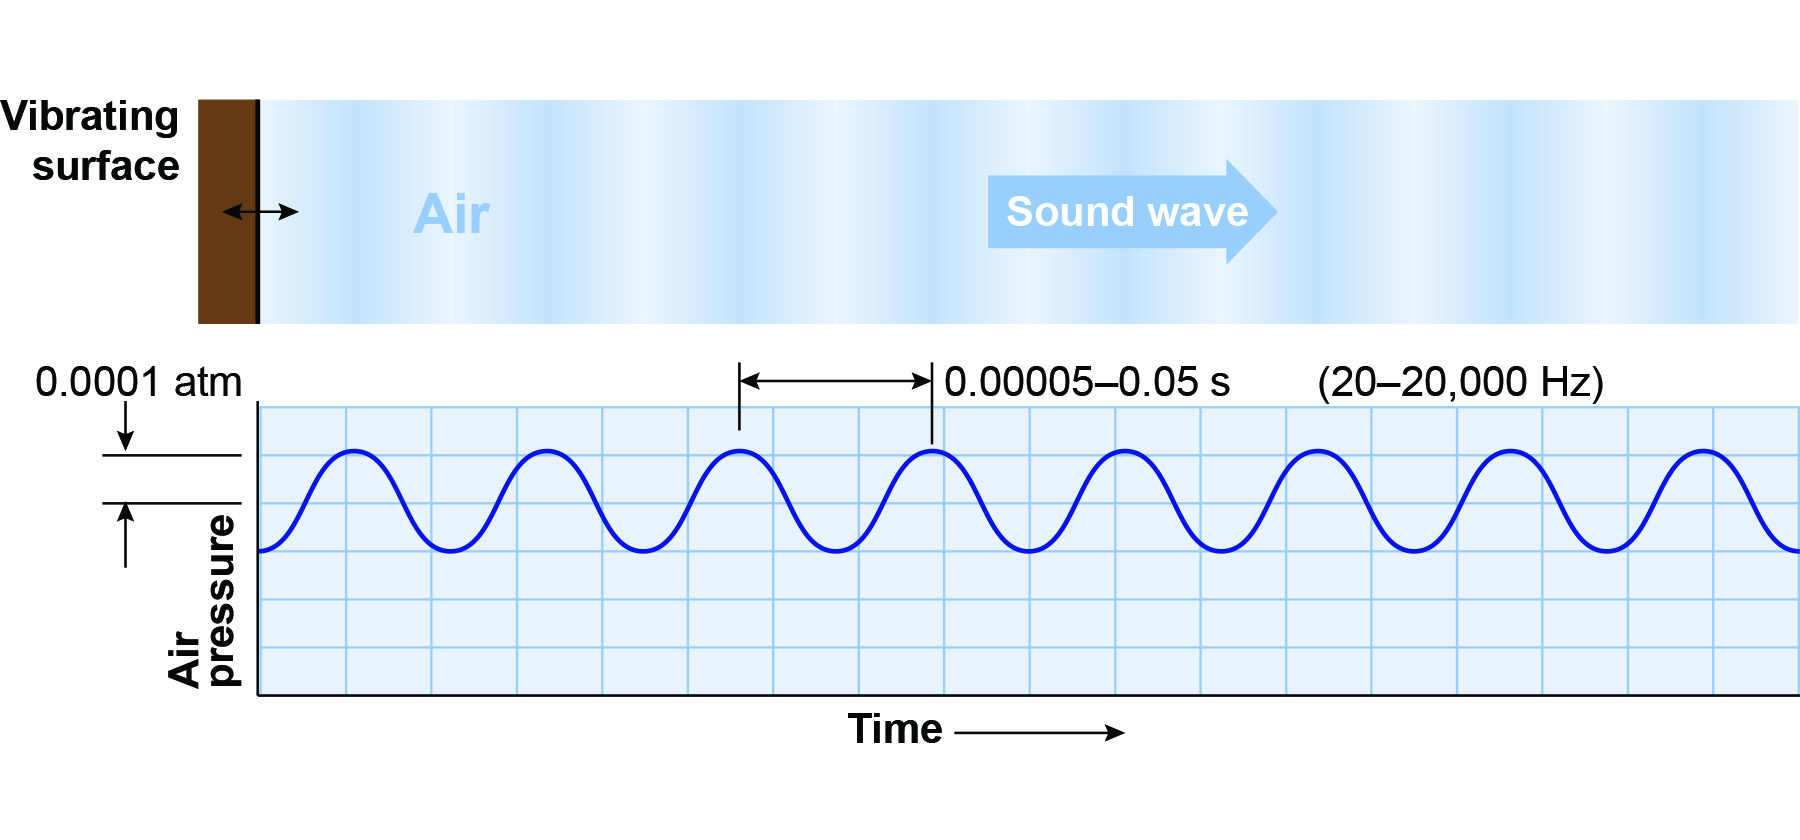
\includegraphics[width=0.8\textwidth]{airpressure}
    \ref{fig:airpressure}
  \begin{center}
  slika 1
  \end{center}
    \section{Počeci snimanja zvuka}
    \label{sec:Počeci snimanja zvuka}
    \subsection {Analogni zapis zvuka}
    U početku je snimanje zvuka bilo analogno, odnosno, zapisivale su se vibracije koje ljudsko uho prepoznaje kao zvuk na neku vrstu medija. 
    Prvi zvuk je snimljen uz pomoć fonoautografa \cite{fonoautograf} sredinom 19. veka. Zatim, Emile Berliner je 1889. godine osmislio gramofon \cite{gramofon} koji je mogao da reprodukuje zvuk gotovo 4 minuta. Edison je 1927. patentirao ploču
    koja je mogla da snima 40 minuta zvučnog zapisa, ali se nije proslavio njom. Godine 1928. Fritz Pfleumer je izumeo magnetnu traku \cite{magnetna traka} i ovaj način snimanja se koristio za vreme Drugog svetskog rata.Nakon toga se pojavila
    stereo magnetna traka koja se mogla koristiti u kućnoj upotrebi. Kompaktna traka i uređaj koji snima i reprodukuje zvuk sa kasete su se pojavili 1964. godine.Kompanija Sony je krajem 80-ih godina predstavila
    novi proizvod DAT (engl.\textit {digital audio tape} ).Ovaj proizvod je prihvaćen od strane raznih industrija jer je mnogo manji od svih prethodnih.
    \subsection {Digitalni zapis zvuka}
    Prvi pokušaj da se kompjuterske obrade zvuka koji je doveo do uspešne digitalne
    transformacije zvuka desio se početkom 1969. godine u Bel Laboratoriji (\textit {Bell
    Labs}), gde je uspešno proizveden veštački, kompjuterski generisan zvuk. U to vreme su se proizvodili PCM \cite{pcm} procesori. Oni su pretvarali zvuk u digitalni zapis, pa je napravljen eksperimentalni laserski disk. Zatim, početkom 80-ih, pojavljuju se kompaktni diskovi nepristupačne cene, što se ubrzo menja. Patentirani su kompaktni diskovi (CD-RW) \cite{cd-rw} koji imaju mogućnost pisanja i brisanja podataka. Napokon, javlja se uređaj koji može da reprodukuje zapisani zvučni zapis - MP3.

\section{Drugi naslov}
\label{sec:naslov2}

Ovde pišem tekst. 
Ovde pišem tekst. 
Ovde pišem tekst. 
Ovde pišem tekst. 

\subsection{... podnaslov}
\label{subsec:podnaslovN}

Ovde pišem tekst. 
Ovde pišem tekst. 
Ovde pišem tekst. 
Ovde pišem tekst. 
Ovde pišem tekst. 
Ovde pišem tekst. 

\section{Ciljevi digitalizacije}
\label{sec:naslovN}

Ciljevi digitalizcije se razlikuju u zavisnosti od toga zašto se primenjuje, želi li se digitalizacijom zaštititi izvorno gradivo ili omogućiti pristup gradivu. S obzirom na današnju tehnologiju, dolazi se u mogućnost „izrade“ sadržaja kome se može bolje i jednostavnije pristupiti kroz deljenje sadržaja institucije preko interneta s mnogobrojnim korisnicima istovremeno. Korisnici očekuju aktivno vođenje stranica ustanova i društvenih mreža kako bi mogli da preslušaju određeni zvučni sadržaj bez fizičkog dolaska u ustanovu.
 
Ustanove digitalizuju svoje gradivo iz sledećih razloga:

\begin{itemize}
  \item kao plaćenu uslugu,
  \item kako bi dodale novi sadržaj u već postojeću zbirku (npr. priče, legende, bajke i sl.),
  \item vezano uz dokumentacijske procese,
  \item vezano uz internet stranicu
  \item radi konzervacije i restauracije,
  \item zbog ulaganja u nove tehnologije.
\end{itemize}

\section{Dobrobiti digitalizacije}
\label{sec:naslovM}

Digitalizacija se danas koristi sve više. Postaje skoro nepojmljivo da određena prodavnica nema bar internet stranicu, dok je to obavezni minimum koji se očekuje od većih kompanija i državnih institucija. Od elektronskih dnevnika, elektronskog bankarstva, društvenih mreža pa sve do muzočkih biblioteka sa milionima pesama, posledice digitalizacije vidimo na svakom koraku. 
Digitalizacija se koristi sve više. Postaje skoro nepojmljivo da određena prodavnica nema bar internet stranicu, dok je to obavezni minimum koji se očekuje od većih kompanija i državnih institucija. Od elektronskih dnevnika, elektronskog bankarstva, društvenih mreža pa sve do muzočkih biblioteka sa milionima pesama, posledice digitalizacije vidimo na svakom koraku. 

Pre digitalizacije, mnogi podaci, informacije, sadržaji su bili znatno skuplji, teže pristupačni, ograničenog broja i upotrebe. Ako bismo hteli da odslušamo novi album odrešenog izvošača, računar ili telefon je sve što nam je potrebno. Za veliki broj slučajeva, ne bismo morali da platimo, ne bismo imali uslov koliko puta smemo i koliko nas sme da sluša taj sadržaj. 
 
Vrlo bitan aspekt digitalizacije je katalogizacija. Zahvaljujući pravilnom arhiviranju i indeksiranju, imamo jasniji pregled i razumevanje sadržaja koje nam štedi vreme pri potrazi za odredjenim podacima, tokom obrade i rukovođenjem.
\section{Zaključak}
\label{sec:zakljucak}

Zvuk su mehaničke vibracije, a čovek prosečnog sluha može da registruje iz intervala 16 - 20 000 Hz. Početkom 19. veka su nastali analogne mašine kojima se mogao zabeležiti zvuk, od kojih je jedan primer gramofon. Upotreba gramofona nije bila preterano skupa, medjutim, ploče preko kojih se čuvao zvuk su bili krhki, osetljivi na temperaturu i tokom svakog koriščenja, štetio se reljef i gubili su se podaci. Nakon gramofona, dolazi do izuma magnetne trake, zatim kompaktne trake i konačno optičkih diskova. Optički diskovi se zarayziku od prethodno navedenih tehnologija nisu habali tokom reprodukcije i primene, al je moglo doći do grebanja tokom držanja i neobazrivog rukovođenja.

Zvučni zapisi sa analognih nosača se mogu  zaštititi od propadanja i učiniti dostupnim većem broju korisnika procesom digitalizacije. Digitalizovane zapise možemo spremiti u više
formata, a najpoznatiji su MP3, AIFF i WAV. Razlika među zapisima je u kvaliteti zapisa. WAV i AIFF su nekompresovani i kvalitetniji upravo jer ne dolzi do gubljenja podataka, kao kod kompresovanog MP3 zapisa. Nadalje, kako bi digitalizovani
zvuk bio zadovoljavajućeg kvaliteteta, potrebno je paziti na frekvenciju uzorkovanja, koja mora biti dvostruko veća od najviše frekvencije kako ne bi došlo do naoštravanja signala. Jedna metoda koja se koristi kako bi se to izbeglo je korišćenje antialiasing filtera, odnosno nisko
propusnog filtera kojim se „odrezuju“ visoke frekvencije. Kvantizacija je isto tako važan deo digitalizacije, pa i od nje zavisi kvalitet zvučnog zapisa. Važan je pojam dubina bita jer što je broj bitova veći, veći je i kvalitet.

Potrebno je digitalizirati gradivo, pogotovo kulturnu baštinu kako se identitet i kultura ne bi zaboravili i kako bi ljudi, odnosno korisnici, digitalizirano gradivo mogli da koriste i tokom celog života. S obzirom na današnju tehnologiju potrebno je i održavati gradivo u određenim formatima kako bi bili čitljivi i dostupni većem broju ljudi.
Analogni izvornici ili izvorno digitalno gradivo će uvek imati svoju vrednost u pogledu informacija.

\addcontentsline{toc}{section}{Literatura}
\appendix

\iffalse
\bibliography{seminarski} 
\bibliographystyle{plain}
\fi

\begin{thebibliography}{9}

\bibitem{laski2009software} J. Laski and W. Stanley. \emph{Software Verification and Analysis}. Springer- Verlag, London, 2009.

\bibitem{gcc} Free Software Foundation. GNU gcc, 2013. on-line at: http://gcc. gnu.org/.

\bibitem{haltingproblem} A. M. Turing. \emph{On Computable Numbers, with an application to the Entscheidungsproblem}. Proceedings of the London Mathematical Society, 2(42):230–265, 1936.




\bibitem{fonoautograf}Fonoautograf. Dostupno na adresi https://griffonagedotcom.wordpress.com/2016/05/25/the-first-phonautograph-in-america-1859/ .

\bibitem{gramofon}Gramofon. Dostupno na adresi https://ia800708.us.archive.org/view_archive.php?archive=/22/items/crossref-pre-1909-scholarly-works/10.1109%252Fpaiee.1909.6660362.zip&file=10.1109%252Ft-aiee.1891.5570135.pdf .

\bibitem{magnetna traka}Magnetne trake. Dostupno na adresi https://www.aes.org/images/e-lib/thumbnails/5/1/5136_full.png .
\bibitem{pcm}PCM. Dostupno na adresi https://www.aes.org/e-lib/browse.cfm?elib=12991 .

\bibitem{cd-rw}CD-RW. Dostupno na adresi https://www.mdpi.com/1424-8220/18/7/2070/html .


\bibitem{}http://www.sveti-sava.edu.rs/otpremljeno/Digitalizacija1.pdf

\bibitem{}https://repozitorij.ffzg.unizg.hr/islandora/object/ffzg%3A4007/datastream/PDF/view





\end{thebibliography}


\appendix
\section{Dodatak}
Ovde pišem dodatne stvari, ukoliko za time ima potrebe.
Ovde pišem dodatne stvari, ukoliko za time ima potrebe.
Ovde pišem dodatne stvari, ukoliko za time ima potrebe.
Ovde pišem dodatne stvari, ukoliko za time ima potrebe.
Ovde pišem dodatne stvari, ukoliko za time ima potrebe.


\end{document}
